%%%%%%%%%%%%%%%%%%%%%%%%%%%%%%%%%%%%%%%%%
% Template Original author:
% Frits Wenneker (http://www.howtotex.com)
%
% License:
% CC BY-NC-SA 3.0 (http://creativecommons.org/licenses/by-nc-sa/3.0/)
%%%%%%%%%%%%%%%%%%%%%%%%%%%%%%%%%%%%%%%%%

%----------------------------------------------------------------------------------------
%	PACKAGES AND OTHER DOCUMENT CONFIGURATIONS
%----------------------------------------------------------------------------------------

\documentclass[fontsize=11pt]{scrartcl} % A4 paper and 11pt font size

\usepackage[T1]{fontenc} % Use 8-bit encoding that has 256 glyphs
\usepackage{fourier} % Use the Adobe Utopia font for the document - comment this line to return to the LaTeX default
\usepackage[english]{babel} % English language/hyphenation
\usepackage{amsmath,amsfonts,amsthm} % Math packages

\usepackage{lipsum} % Used for inserting dummy 'Lorem ipsum' text into the template

\usepackage{sectsty} % Allows customizing section commands
\allsectionsfont{\centering \normalfont\scshape} % Make all sections centered, the default font and small caps

\usepackage{fancyhdr} % Custom headers and footers
\pagestyle{fancyplain} % Makes all pages in the document conform to the custom headers and footers
\fancyhead{} % No page header - if you want one, create it in the same way as the footers below
\fancyfoot[L]{} % Empty left footer
\fancyfoot[C]{} % Empty center footer
\fancyfoot[R]{\thepage} % Page numbering for right footer
\renewcommand{\headrulewidth}{0pt} % Remove header underlines
\renewcommand{\footrulewidth}{0pt} % Remove footer underlines
\setlength{\headheight}{13.6pt} % Customize the height of the header

\numberwithin{equation}{section} % Number equations within sections (i.e. 1.1, 1.2, 2.1, 2.2 instead of 1, 2, 3, 4)
\numberwithin{figure}{section} % Number figures within sections (i.e. 1.1, 1.2, 2.1, 2.2 instead of 1, 2, 3, 4)
\numberwithin{table}{section} % Number tables within sections (i.e. 1.1, 1.2, 2.1, 2.2 instead of 1, 2, 3, 4)

\setlength\parindent{0pt} % Removes all indentation from paragraphs - comment this line for an assignment with lots of text

\usepackage{tikz}
\tikzset{main node/.style={circle,fill=blue!20,draw,minimum size=1cm,inner sep=0pt},
}
\usetikzlibrary{positioning}
%----------------------------------------------------------------------------------------
%	TITLE SECTION
%----------------------------------------------------------------------------------------

\newcommand{\horrule}[1]{\rule{\linewidth}{#1}} % Create horizontal rule command with 1 argument of height

\title{	
\normalfont \normalsize 
\textsc{George Washington University, Department of Mathematics} \\ [25pt] % Your university, school and/or department name(s)
\textsc{Graph Theory, MATH 3632}
\horrule{0.5pt} \\[0.4cm] % Thin top horizontal rule
\huge Problem Set I \\ % The assignment title
\horrule{2pt} \\[0.5cm] % Thick bottom horizontal rule
}

\author{Joseph Espy} % Your name

\date{\normalsize\today} % Today's date or a custom date

\begin{document}

\maketitle % Print the title

%----------------------------------------------------------------------------------------
%	PROBLEM 1
%----------------------------------------------------------------------------------------

\section*{Exercise I}

It is known that a certain statement $Q(n)$ satisfies the following conditions:
		\begin{labeling}{a}
			\item[(a)] $Q(1001)$ is true.
			\item[(b)] If $n \geq 4$ and $Q(n)$ is true, then so is $Q(n-3)$.
			\item[(c)] If $Q(n)$ is true, then so is $Q(2n)$.
		\end{labeling}
		
		For what $n \in \mathbb{N}$ can you conclude that $Q(n)$ is true?\\
		
		$Q(n)$ is true in every case $n \in \mathbb{N} \geq 1 $ where $ n \equiv_3 2 \lor n \equiv_3 2 $.  I will prove by cases:
		
		\begin{itemize}
			\item whenever $n \equiv_3 2$, $Q(n)$ must be true:\\
			$1001 \equiv_3 2$ because $1001 - (3\cdot111) = 2$.  So $Q(2)$ is true by (a) and (b)\\
			We can obtain an arbitrarily large $k$ for which $Q(k)$ is true and $k \equiv_3 2$ by iteratively multiplying 2 (our base) by 4.  \\
			$Q(k)$ will be true after successive multiplications by $4$ because of (c). \\
			$k \equiv_3 2$ by the rules of modular arithmetic ($4\equiv_3 1$)\\
			So for any $n\equiv_3 2$, we can produce a larger value $k$ which is true.  And after iteratively subtracting 3 from that value, we get $n$.  \\
			by (b), $Q(n)$ is true\\
			
			\item whenever $n \equiv_3 1$, $Q(n)$ must be true:\\
			From the above result, $Q(4)$ is true, ans so it follows from (b) that $Q(1)$ is true\\
			For the same reason as the above proof, we can create an arbitrarily large $k \equiv_3 1$ by successively multiplying $1$ by $4$\\
			Finally, we can obtain $Q(n)$ for any $n \equiv_3 1$ by successively subtracting $3$ from an arbitrarily large $k$\\
			
			\item It is not possible to prove that $Q(n)$ is true (or false) from the statements provided where $n \equiv_3 0$.  (a) only gives a specific value which does not happen to be $\equiv_3 0$.  (b) provides a relation for finding new values for which $Q(m)$ is true given $Q(n)$ is true, however the relation is only goes between values of the same modular 3 equivalence class.  (c) similarly finds a method for finding new values, however if the known value $Q(n)$ is $\equiv_3 2$ then the found result will be $\equiv 3 1$, and vice versa.  The only way to use this rule to find a value $\equiv_3 0$ is by already knowing a value for which it is true.  So there is no way to reason about $Q(n)$ where $n \equiv_3 0$.  
		\end{itemize}

\section*{Exercise II}
	For every $k$-regular graph is there a $(k+1)$-regular graph that contains the $k$-regular graph as a subgraph?\\
	
	Yes.  Each k-regular graph is a subset of $K_{k+2}$.  $K_{k+2}$ is $(k+1)$-regular and has as a subset, every $k$-regular graph 


\section*{Exercise III} Which, if any, of the graphs $G_1$, $G_2$, and $G_3$ in the figure below are isomorphic? For those that are isomorphic, construct an isomorphism between them; for those that are not, state a graph-theoretic property satisfied by one and not the other. \\
		
		None of these graphs are isomorphic to another.  Graph $G_1$ cannot be isomorphic to either of the others because it has $|G_1(E)| = 12$ while the other two graphs have $|G_2(E)| = 14$ and $|G_3(E)| = 14$.\\  
		
		Graph $G_2$ is not isomorphic to graph $G_3$ because there exists a closed trail $\{v_0, e_1, v_1 ... e_4, v_0\}$ (length of 4 edges, begins and ends at the same vertex), where the only one of the four vertexes has a degree of 3, and the other four have degree of four.  An example of this in graph $G_2$ stars at the vertex lowest on the page (of degree 3), follows the edge up and to the right (degree 4), follows directly up (degree 4), follows down and to the left, to the leftmost vertex in the bottom row of three (four edges), and then returns to the starting point (bottom vertex of degree 3).  \\
		
		By an exhaustive search of $G_3$, there is no path of length 4 beginning and ending at the same location with three 4-degree vertexes and a single 3-degree vertex

\section*{Exercise IV}
			If a simple graph $G$ is isomorphic to its complement $\overline G$, then $G$ has either $4k$ or $4k+1$ vertexes for some $k \in \mathbb{N}$.  Find all simple graphs in on four and five vertexes that are isomorphic to their complements.\\
			
			The the only graph on 4 vertexes which is isomorphic to its own complements is:
			
			
			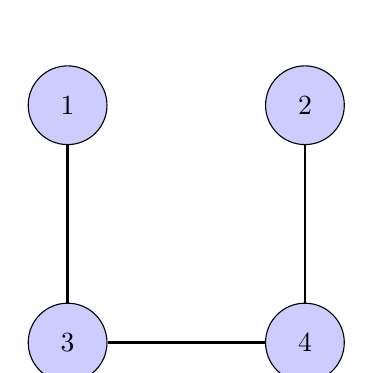
\begin{tikzpicture}

			%%
			\begin{scope}[xshift=4cm]
			\node[main node] (1) {$1$};
			\node[main node] (2) [right = 2cm  of 1]  {$2$};
			\node[main node] (3) [below = 2cm  of 1] {$3$};
			\node[main node] (4) [right = 2cm  of 3] {$4$};
			
			\path[draw,thick]
			(1) edge node {} (3)
			(3) edge node {} (4)
			(4) edge node {} (2)
			;
			\end{scope}
			\end{tikzpicture}
			
			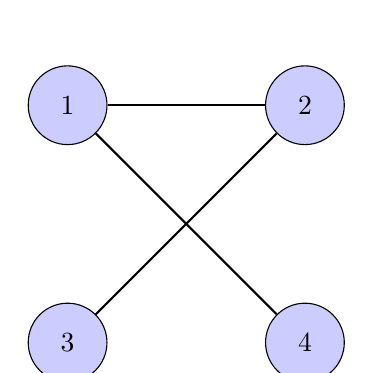
\begin{tikzpicture}
			
			%%
			\begin{scope}[xshift=4cm]
			\node[main node] (1) {$1$};
			\node[main node] (2) [right = 2cm  of 1]  {$2$};
			\node[main node] (3) [below = 2cm  of 1] {$3$};
			\node[main node] (4) [right = 2cm  of 3] {$4$};
			
			\path[draw,thick]
			(1) edge node {} (2)
			(1) edge node {} (4)
			(3) edge node {} (2)
			;
			\end{scope}
			\end{tikzpicture}
			
			The only two graphs on five vertexes which are isomorphic to their own complements are:
			
			
			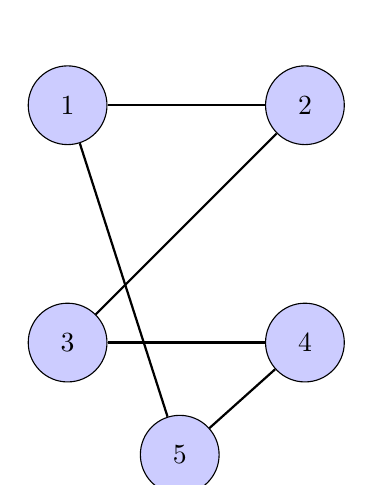
\begin{tikzpicture}
			
			%%
			\begin{scope}[xshift=4cm]
			\node[main node] (1) {$1$};
			\node[main node] (2) [right = 2cm  of 1]  {$2$};
			\node[main node] (3) [below = 2cm  of 1] {$3$};
			\node[main node] (4) [right = 2cm  of 3] {$4$};
			\node[main node] (5) [below right = 1cm  of 3] {$5$};
			
			\path[draw,thick]
			(1) edge node {} (2)
			%(1) edge node {} (3)
			%(1) edge node {} (4)
			(1) edge node {} (5)
			(2) edge node {} (3)
			%(2) edge node {} (4)
			%(2) edge node {} (5)
			(3) edge node {} (4)
			%(3) edge node {} (5)
			(4) edge node {} (5)
			;
			\end{scope}
			\end{tikzpicture}

			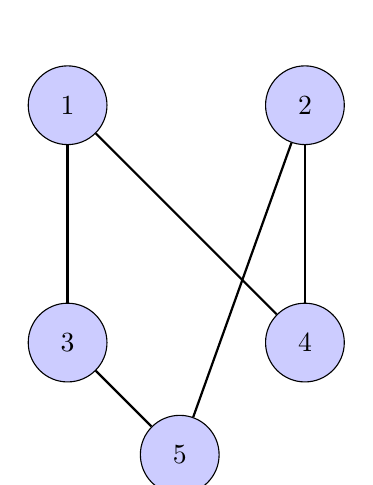
\begin{tikzpicture}
			
			%%
			\begin{scope}[xshift=4cm]
			\node[main node] (1) {$1$};
			\node[main node] (2) [right = 2cm  of 1]  {$2$};
			\node[main node] (3) [below = 2cm  of 1] {$3$};
			\node[main node] (4) [right = 2cm  of 3] {$4$};
			\node[main node] (5) [below right = 1cm  of 3] {$5$};
			
			\path[draw,thick]
			%(1) edge node {} (2)
			(1) edge node {} (3)
			(1) edge node {} (4)
			%(1) edge node {} (5)
			%(2) edge node {} (3)
			(2) edge node {} (4)
			(2) edge node {} (5)
			%(3) edge node {} (4)
			(3) edge node {} (5)
			%(4) edge node {} (5)
			;
			\end{scope}
			\end{tikzpicture}	
			
			The second graph and its isomorphic complement is:	
			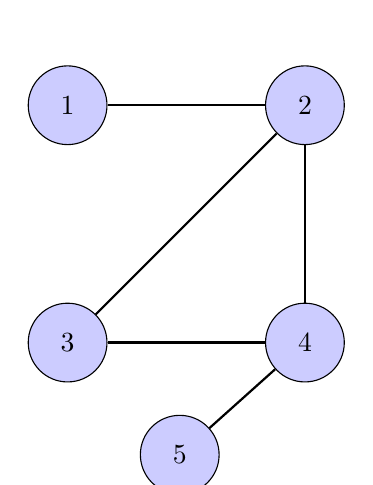
\begin{tikzpicture}
			
			%%
			\begin{scope}[xshift=4cm]
			\node[main node] (1) {$1$};
			\node[main node] (2) [right = 2cm  of 1]  {$2$};
			\node[main node] (3) [below = 2cm  of 1] {$3$};
			\node[main node] (4) [right = 2cm  of 3] {$4$};
			\node[main node] (5) [below right = 1cm  of 3] {$5$};
			
			\path[draw,thick]
			(1) edge node {} (2)
			%(1) edge node {} (3)
			%(1) edge node {} (4)
			%(1) edge node {} (5)
			(2) edge node {} (3)
			(2) edge node {} (4)
			%(2) edge node {} (5)
			(3) edge node {} (4)
			%(3) edge node {} (5)
			(4) edge node {} (5)
			;
			\end{scope}
			\end{tikzpicture}
			
			and 
						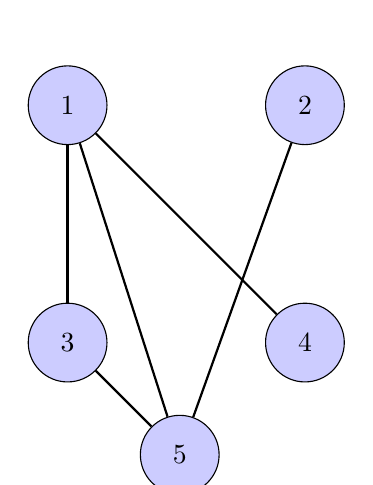
\begin{tikzpicture}
						
						%%
						\begin{scope}[xshift=4cm]
						\node[main node] (1) {$1$};
						\node[main node] (2) [right = 2cm  of 1]  {$2$};
						\node[main node] (3) [below = 2cm  of 1] {$3$};
						\node[main node] (4) [right = 2cm  of 3] {$4$};
						\node[main node] (5) [below right = 1cm  of 3] {$5$};
						
						\path[draw,thick]
						%(1) edge node {} (2)
						(1) edge node {} (3)
						(1) edge node {} (4)
						(1) edge node {} (5)
						%(2) edge node {} (3)
						%(2) edge node {} (4)
						(2) edge node {} (5)
						%(3) edge node {} (4)
						(3) edge node {} (5)
						%(4) edge node {} (5)
						;
						\end{scope}
						\end{tikzpicture}
						
	

\section*{Exercise V}
 For which values of $n$, $r$ is there an $r$-regular graph on $n$ vertexes? An
	$r$-regular simple graph?\\
	
	There is always an r-regular graph on n vertexes.  One can construct such a graph by putting r self-loops on n vertexes.  
	
	There are no r-regular graphs on n vertexes for an $r \geq n$ because a fully connected graph has $n-1$ edges to a node, and another edge cannot be added without becoming non-simple.  Below this, I restrict $r< n$.  
	
	For non-simple graphs, by the handshake theorem, if both n and r are odd, there cannot be an r regular graph on n vertexes.  The sum of all of the edges for each vertex must be even, because each edge is attached to two vertexes.  \\
	
	For any even n, there is an $r$ regular graph on n vertexes.  You can construct this by taking $K_n$, splitting the graph into connected pairs, and removing the end from that pair.  Repeat this until the graph is $r$ regular.  \\
	
	For an odd n and even r, $C_5$ is 2-regular on 5 vertexes.  So there exist some.  I believe that there exist some for any n and r.  


\section*{Exercise VI}

 Consider the Knight's Graph on an $n \times n$ chessboard:\\ 
	\begin{enumerate}
		\item[$a$)] For which $n$ is it connected?
		\item[$b$)] For which $n$ is it Eulerian?
		\item[$c$)] For which $n$ does it have $K_3$ as a subgraph?
	\end{enumerate}
$n$ is connected for any $n \geq 4$.  Consider a subroutine to move one unit in a specific direction: first move two units in the goal direction and one unit up or down.  next move one unit in the the opposite non-goal direction and two units away from the goal direction.  You are now either two units above or below where you began.  From there, move to the position one unit in the goal direction from your starting place.  \\

Using this subroutine, you can visit every position in a 3x3 board assuming that you are able to move within a larger 4x4 board.  \\


from a connected 3x3 board, you can get to any position in a larger 4x4 board by moving from a 2-interior position to the exterior position.  You can iteratively do this, so by induction, any $n>3$ board is connected.  \\

It is not connected for $n \leq 3$.  when $n = 3$ the middle position is unreachable, and when less, no new positions are reachable.  $n=1$ is vacuously connected.  \\

There is only an Eulerian cycle for $n=1$, because there are no edges.  For $n=2,3$ it is not connected.  For $n\geq 4$, there are an even number of nodes with odd degree.  The edge positions which are adjacent to corners can each make three moves.  There are 8 of these position.  \\

There is no $K_3$ subgraph.  The knight will have moved twice, and will either be on a row/column with its original position, and unable to reach the starting point, or three or greater steps on one of the directions, so unable to reach its starting point.  So there is no subgraph that starts and ends in the same location and has only three edges.  

\section*{Exercise VII}

	\begin{itemize}
		\item[$a$)] 
			There is no simple graph on $n > 1$ vertices with all vertex degrees distinct.

		\item[$b$)] What if we drop the adjective ``simple"?
		\item[$c$)] \textbf{Extra credit:} characterize all simple graphs that have a single pair
		of vertices with the same degree, and all other degrees distinct.
	\end{itemize}
	
	By contradiction, there is no simple graph on $n > 1$ vertices with all distinct vertex degrees.  Consider the simple graph on $n$ vertices with all distinct vertex degrees. The first vertex has at least 0 edges, the second has at least 1 edge... until the nth vertex with at least $n-1$ edges.  However the no vertex can have more than $(n-2)$ edges, as there are only $n-2$ other edges to connect to (if the first vertex is not connected to anything).  So there are n vertexes edge values which are distinct between $0$ and $n-2$ (if the first vertex is connected, n vertexes between $1$ and $n-1$).  By the pigeon hole principal, two vertexes must have the same number of edges.  \\
	
	If we drop 'simple', then this is easy to construct.  The first vertex has 0 edges, the second has 1 edge is only connected to itself... the $n$th vertex has $n-1$ self loops.  

\section*{Exercise VIII}
	Suppose that the graph $G-v$ is connected for every vertex $v$ of $G$.
	Does it follow that $G$ is connected? (Be comprehensive.)\\

If the size of $2$ is 2 or less, then the graph my not be connected.  Consider two vertexes not connected.  The graph $G-v$ is not connected but $G$ is connected.  However whenever the size of $V$ is more than two, the statement is true.  

\section*{Exercise IX}
 Show that if a simple graph $G$ has an odd cycle as a subgraph, it also
	has an odd cycle as an $induced$ subgraph. Is the same true if` `odd? is
	replaced by ``even??\\
	
	If not every node in the graph $G$ is on the odd cycle, then choose a node not on the odd cycle, and remove it.  That induced subgraph has the same odd cycle.  \\
	
	If every node in the graph is on the odd cycle, then there is an additional edge between two elements on the odd cycle (or else it would not be a subgraph, I am assuming strict subgraph).  That edge creates two 'sub-cycles'.  The length of the first subcyle $-1$ plus the length of the second subcycle $-1$ is the length of the original odd cycle.  So it follows that one of the new subcycles is of odd length.  So choose an element not on the odd subcycle, and remove that.  So the induced graph must have an odd cycle.  

\section*{Exercise X}
\begin{itemize}
		\item[$a$)] 
		If a graph $G$ has a closed walk of odd length then it has
			an odd cycle as a subgraph.
		
		\item[$b$)] Nevertheless, give a counter-example to exercise 2.3: if $G$ contains a closed trail of length seven, then $G$ contains some $C_3$, $C_5$, ... or $C_7$ as a subgraph?
	\end{itemize}
	
	If the graph $G$ has a closed walk of odd length, then it either is a cycle of odd length, or it has some edge which is repeated in the walk.  If there is a cycle of odd length, then we are finished.  Else, we can remove the repeated edge.  When the edge has been repeated, there are two subwalks created.  The sum of the length of the two subwalks is the length of the original odd walk minus two.  So one of the walks is odd. We can repeat this until we have an odd cycle.  \\
	
	$C_8$ has a closed trail of length 7 and but does not have a subgraph of any $C_n$ where $n \leq 7$  

\end{document}